%! Author = jonathan
%! Date = 5/26/25
\chapter{Introduction}\label{ch:introduction}
State-of-the-art large language models (LLMs), including DeepSeek-v3~\cite{deepep}, LLama4~\cite{llama4},
DBRX~\cite{dbrx} and Snowflake Arctic~\cite{arctic}, have adopted the Mixture-of-Experts (MoE)
~\cite{DBLP:conf/iclr/ShazeerMMDLHD17}
architecture for its computational efficiency~\cite{pmlr-v162-rajbhandari22a} and reliable
performance across language modeling tasks~\cite{deepep, llama4, jiang2024mixtralexperts}.
\begin{figure}[!ht]
    \centering
    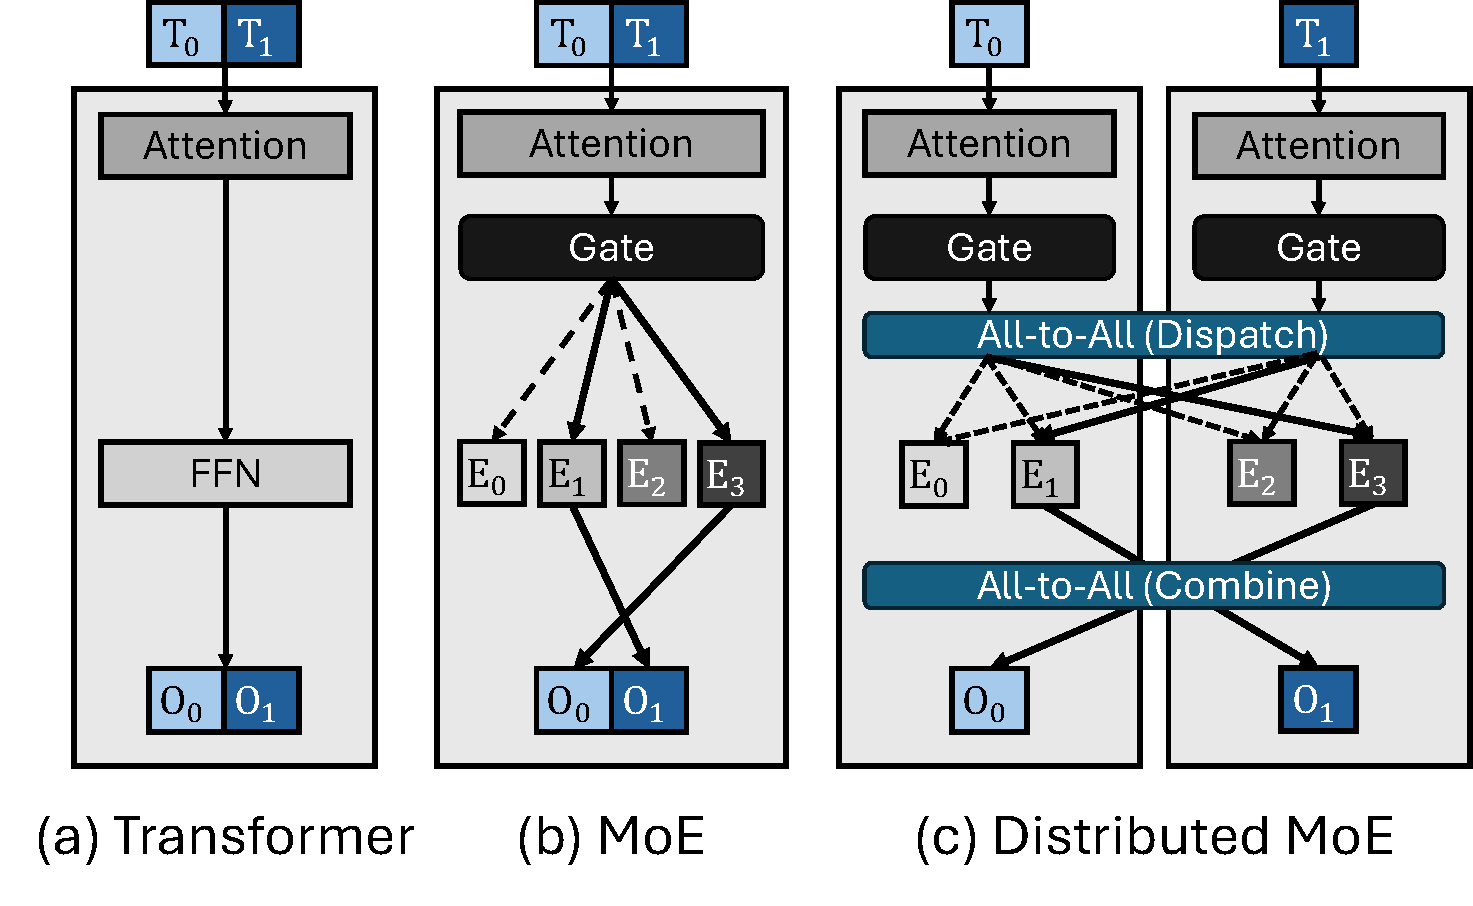
\includegraphics[width=0.55\textwidth, keepaspectratio]{figures/fig-bg-moe}
    \caption{Transformer blocks (a) without MoE, (b) with MoE, and (c) with distributed MoE and expert parallelism.
        \texttt{T}, \texttt{E}, and \texttt{O} represent input tokens, experts, and output activations, respectively.}
    \label{fig:bg:moe}
\end{figure}

Depicted in Figure~\ref{fig:bg:moe}(a), the conventional Transformer block consists of
a self-attention module followed by a feed-forward network (FFN)~\cite{NIPS2017_3f5ee243}.
In contrast, MoE architectures replace this single FFN with identically sized FFNs,
otherwise known as experts, (Figure~\ref{fig:bg:moe}(b)).
A trainable neural network, known as a gate function, sparsely activates these experts by
dynamically routing input tokens to selected experts at runtime.
This increase in model parameters (more FFNs) improves model quality without a
\textit{corresponding increase in computational cost}.
\section{Computational Cost Equivalence}\label{sec:comoutational-cost-equivalence}
The preceding claim seems counterintuitive because \emph{shouldn't the increase in the number of experts
yield a proportional increase in the model's computational operations?}
The answer is no, due to how tokens are \emph{distributed} across experts in comparison to the singular FFN.
For example, consider a token matrix $T$ as defined below where $S$ is the sequence length and $H$
the embedding dimension.
\[
    T \in \mathbb{R}^{S \times H}
\]
The typical FFN operator, defined below,
\begin{equation}\label{eq:ffn}
\textrm{FFN}(x) = W_2 \cdot \phi(x W_1 + b_1) + b_2
\end{equation}
comprises two linear transformations on learnable weight matrices
$W_1\in \mathbb{R}^{H \times P}$, $W_2 \in \mathbb{R}^{P \times H}$ each followed by additions with bias terms
$b_1 \in \mathbb{R}^{1 \times P}$, $b_2 \in \mathbb{R}^{1 \times H}$ and separated by a
nonlinear activation $\phi$ (e.g., GELU~\cite{hendrycks2023gaussianerrorlinearunits} or
ReLU~\cite{10.5555/3104322.3104425}).
Here dimension $P$ is an intermediate projection for the FFN\@, typically $P = 4\cdot H$~\cite{NEURIPS2024_9f2b171f}.
If we define $\mathcal{F}_{FFN}$ as the \textbf{F}loating \textbf{P}oint \textbf{OP}erations (FLOPs)
needed to compute a forward pass of the FFN, then using Equation~\ref{eq:ffn} we have the resulting expression.
\begin{equation}\label{eq:flopsffn}
\mathcal{F}_{FFN} = \mathcal{F}_{L_0} + \mathcal{F}_{L_1}
\end{equation}
where $\mathcal{F}_{L_i}$ is the FLOPs cost for computing linear transformation $i$.
These linear transformations are \textbf{GE}neral \textbf{M}atrix \textbf{M}ultiplications (GEMMs).
We know that multiplying two matrices of sizes $(M, K)$ and $(K, N)$ demands $2MNK$ FLOPs,
therefore we can expand Equation~\ref{eq:flopsffn} as
\begin{equation}\label{eq:flopsffn2}
\mathcal{F}_{FFN} = 2SHP + 2SHP = 4SHP
\end{equation}

An MoE model differs from the dense transformer by \emph{restricting} the number of
tokens~\cite{DBLP:conf/iclr/LepikhinLXCFHKS21, MLSYS2023_5a54f793} routed to an FFN
(interchangeably called expert).
Specifically, for a model with $N_e$ experts, each expert has a fixed capacity for tokens $S_e$ defined as follows
\begin{equation}\label{eq:capacity}
S_e = \frac{S}{N_e}
\end{equation}
With the above, we can compute $\mathcal{F}_{MoE}$.
Intuitively, this quantity would be the aggregate of $\mathcal{F}_{{FFN}_j}$ where $j \in \{0, \cdots, N_e - 1\}$.
\begin{equation}\label{eq:flopsmoe}
\mathcal{F}_{MoE} = \sum\limits_{j = 0}^{N_e - 1}\mathcal{F}_{{FFN}_j}
\end{equation}
Observe that $\mathcal{F}_{{FFN}_j}$ is derivable from Equation~\ref{eq:flopsffn}
by replacing $S$ with $S_e$.
Applying this observation and evaluating~\ref{eq:flopsmoe} gives the below result
\begin{equation}\label{eq:flopsmoe2}
\mathcal{F}_{MoE} = N_e \cdot 4S_{e}HP
\end{equation}
Substituting with~\ref{eq:capacity}, yields the below which proves that the computational cost is equivalent
between the MoE and dense transformer models!
\begin{equation}\label{eq:equivalence}
\mathcal{F}_{MoE} = 4SHP = \mathcal{F}_{FFN}
\end{equation}
This relationship presents empirically as uniform latency independent of changes in $N_e$
as \sysname and Megatron-\{CUTLASS, TE\} exhibit in Figure~\ref{fig:expert_trend},
where $N_e \in \{8, \cdots, 128\}$.
\begin{figure}[!h]
    \centering
    \begin{subfigure}{0.485\textwidth}
        \centering
        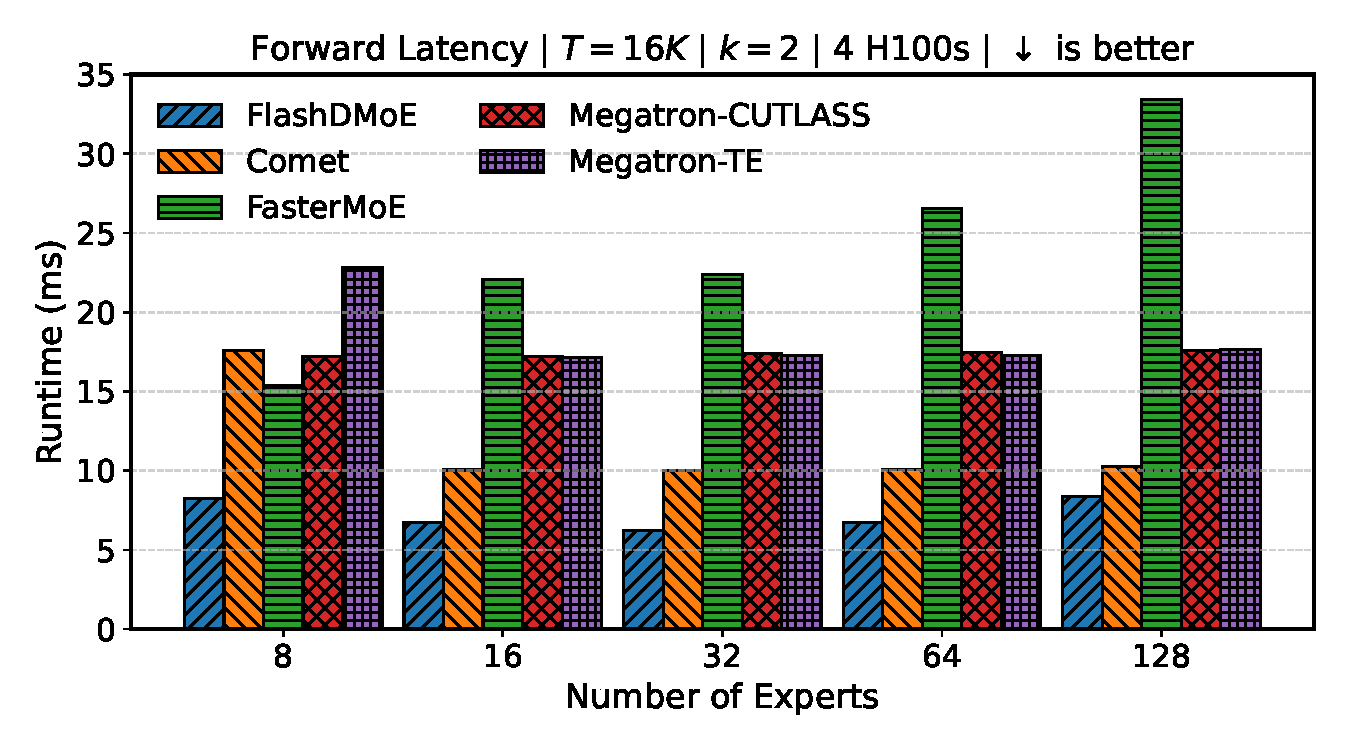
\includegraphics[width=\linewidth, keepaspectratio]{figures/scaling_experts}
        \caption{$4$ H100s}
        \label{sub:4_expert_trend}
    \end{subfigure}
    \begin{subfigure}{0.485\textwidth}
        \centering
        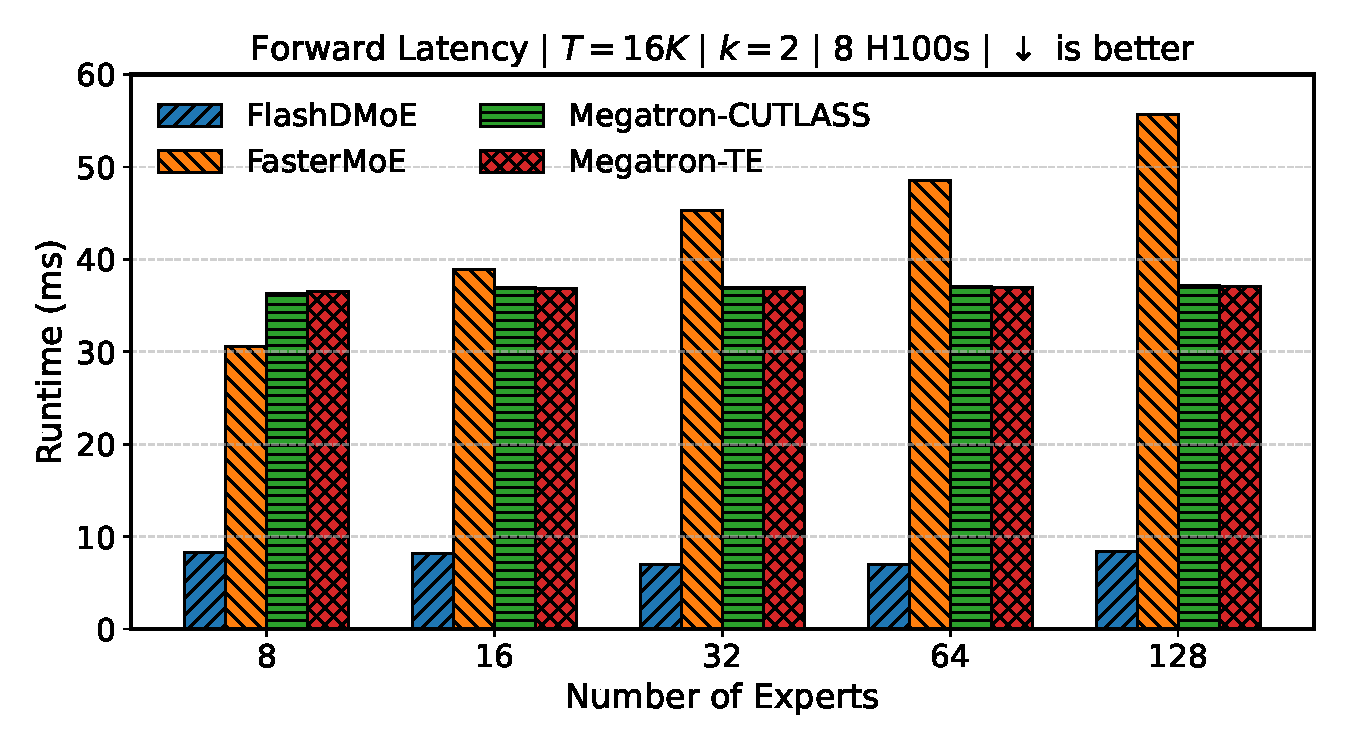
\includegraphics[width=\textwidth, keepaspectratio]{figures/scaling_experts_8}
        \caption{$8$ H100s}
        \label{sub:8_expert_trend}
    \end{subfigure}
    \caption{Correlative trend between forward runtime and number of experts across different MoE operators.}
    \label{fig:expert_trend}
\end{figure}

\section{Communication Overheads in Distributed MoE}\label{sec:communication-overheads-in-distributed-moe}
\begin{figure}[!ht]
    \centering
    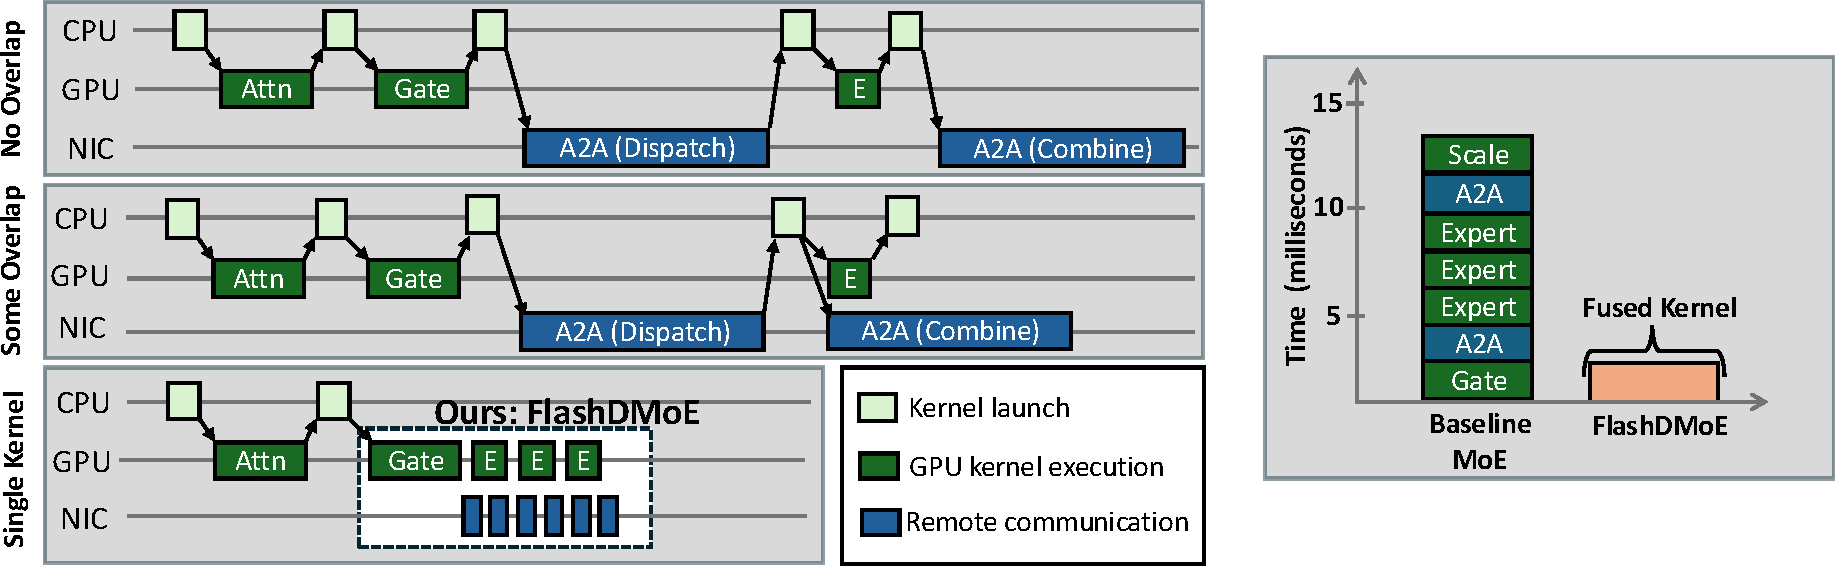
\includegraphics[width=0.98\textwidth, keepaspectratio]{figures/intro-fig}
    \caption{Comparing \sysname with state-of-the-art techniques that either do not overlap communication and
    computation (left, top) or do some overlap (left, middle). \sysname is a persistent kernel that fuses all
    computation and communication of the MoE operator (left, bottom). \sysname implements
    device-initiated computation (gate, expert FFN, scale) and communication tasks (right).}
    \label{fig:intro}
\end{figure}
As MoE model sizes grow, GPU memory constraints prevent hosting all experts on a single device.
The standard practice is to distribute experts across multiple GPUs using expert parallelism (EP),
which requires token routing via many-to-many communication in \alltoall or
\allgather~\cite{deepep, arctic, dbrx, 10.1145/3577193.3593704}.
Another round of said many-to-many communication is also necessary for restoring the permuted tokens processed by experts
to their original order within the sequence.
Existing work has observed these communication operations
taking 68\% of total runtime~\cite{10.1145/3603269.3604869, MLSYS2024_339caf45},
during which the GPU is completely idle, unless the implementation explicitly overlaps with computation.
This form of pipelining is challenging to achieve efficiently because it requires
\emph{asynchronous GPU-driven communication} and \emph{kernel fusion} to maximize the overlap efficiency.
Typically, inter-GPU communication APIs available in frameworks like PyTorch are not of this kind but instead are
\emph{CPU-driven}~\cite{nccl}.
\section{Kernel Launch Overheads in Distributed MoE}\label{sec:kernel-launch-overheads-in-distributed-moe}
\begin{table}[!ht]
    \centering
    \small
    \setlength{\tabcolsep}{8pt}
    \renewcommand{\arraystretch}{0.9}
    \begin{tabular}{@{}lc@{}}
        \toprule
        \textbf{Works} & \textbf{Launched GPU Ops} \\ \midrule
        \sysname & 1 \\
        COMET~\cite{comet} & 33 \\
        Megatron-LM CUTLASS~\cite{megatron, 10.1145/3458817.3476209} & 85 \\
        Megatron-LM TE~\cite{megatron, 10.1145/3458817.3476209} & 261 \\
        Megatron-LM + DeepEP~\cite{deepep} & 432 \\
        DeepSpeedMoE~\cite{pmlr-v162-rajbhandari22a} & 550 \\
        \bottomrule
    \end{tabular}
    \caption{\textbf{Kernel Fusion Comparison.}
    Our method is the first to fully fuse the DMoE layer into a single GPU kernel.
    We report GPU operations from detailed profiling with Nsight Systems.}
    \label{tab:gpuOps}
\end{table}
To mitigate these communication bottlenecks,
recent work pipelines computation with communication tasks
(Figure~\ref{fig:intro}, middle left).
However, The efficacy of communication overlap is further limited by the overhead of
launching many kernels from the CPU\@.
Specifically, existing implementations~\cite{pmlr-v162-rajbhandari22a, comet, megatron, fastermoe}
require launching a large number of kernels per a single layer pass (see Table~\ref{tab:gpuOps}).
Frequent kernel launches negatively affect performance by:
(1) creating non-deterministic kernel start times across GPUs, exacerbating straggler issues;
(2) introducing unnecessary synchronization points, causing GPUs to wait on peers or the CPU before proceeding;
and (3) incurring repeated global memory round trips at kernel boundaries.
Although CUDA graphs~\cite{cuda_graphs_nvidia_blog} can partially mitigate the first issue in static workloads,
they are incompatible with MoE's dynamically shaped tensors.
Addressing the remaining issues requires novel solutions,
which we provide in this work through complete kernel fusion and asynchronous device-initiated communication.
\section{This work's Contributions: Fast DMoE in a single kernel}\label{sec:contributions:-moe-operator-in-a-single-kernel}
\begin{figure}[!h]
    \centering
    \begin{subfigure}{0.4\textwidth}
        \centering
        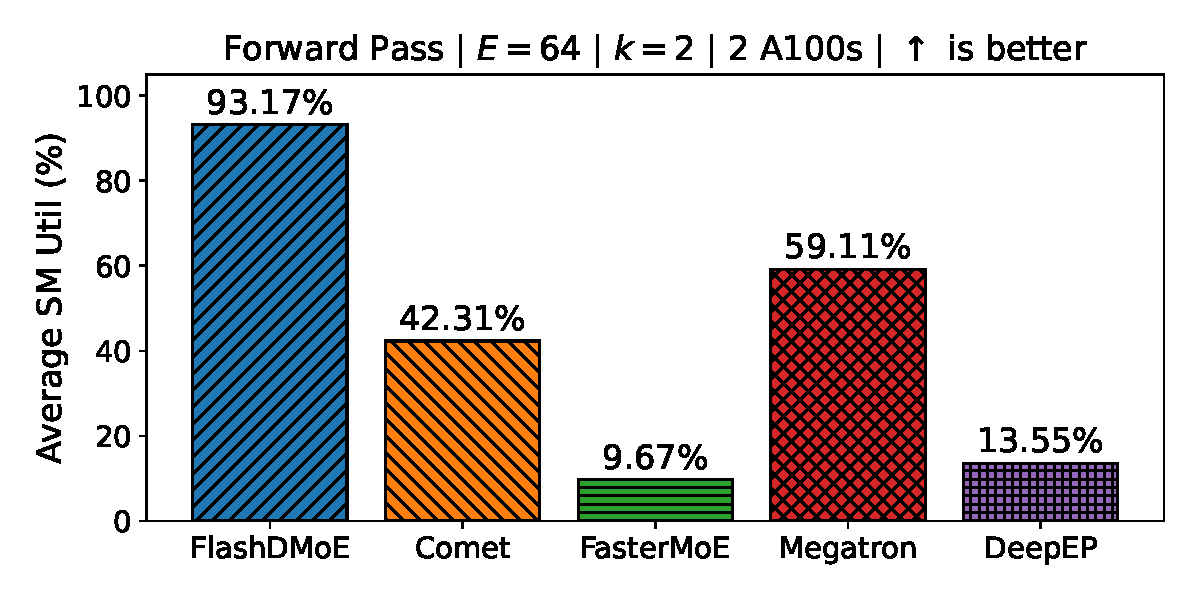
\includegraphics[width=\linewidth, keepaspectratio]{figures/sm_util}
        \caption{GPU SM Utilization}
        \label{sub:util}
    \end{subfigure}
    \begin{subfigure}{0.4\textwidth}
        \centering
        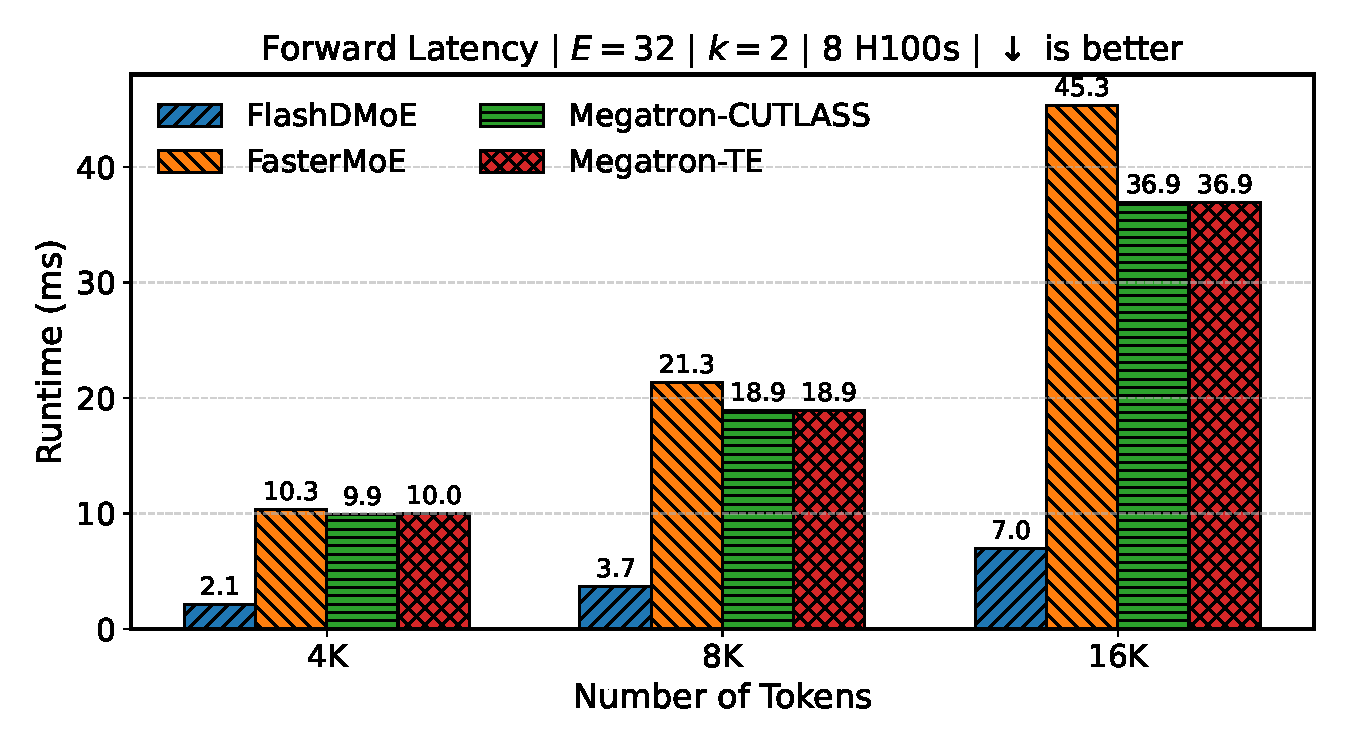
\includegraphics[width=\linewidth, keepaspectratio]{figures/scaling_tokens_8}
        \caption{Scaling Tokens}
        \label{sub:tok}
    \end{subfigure}
    \begin{subfigure}{0.4\textwidth}
        \centering
        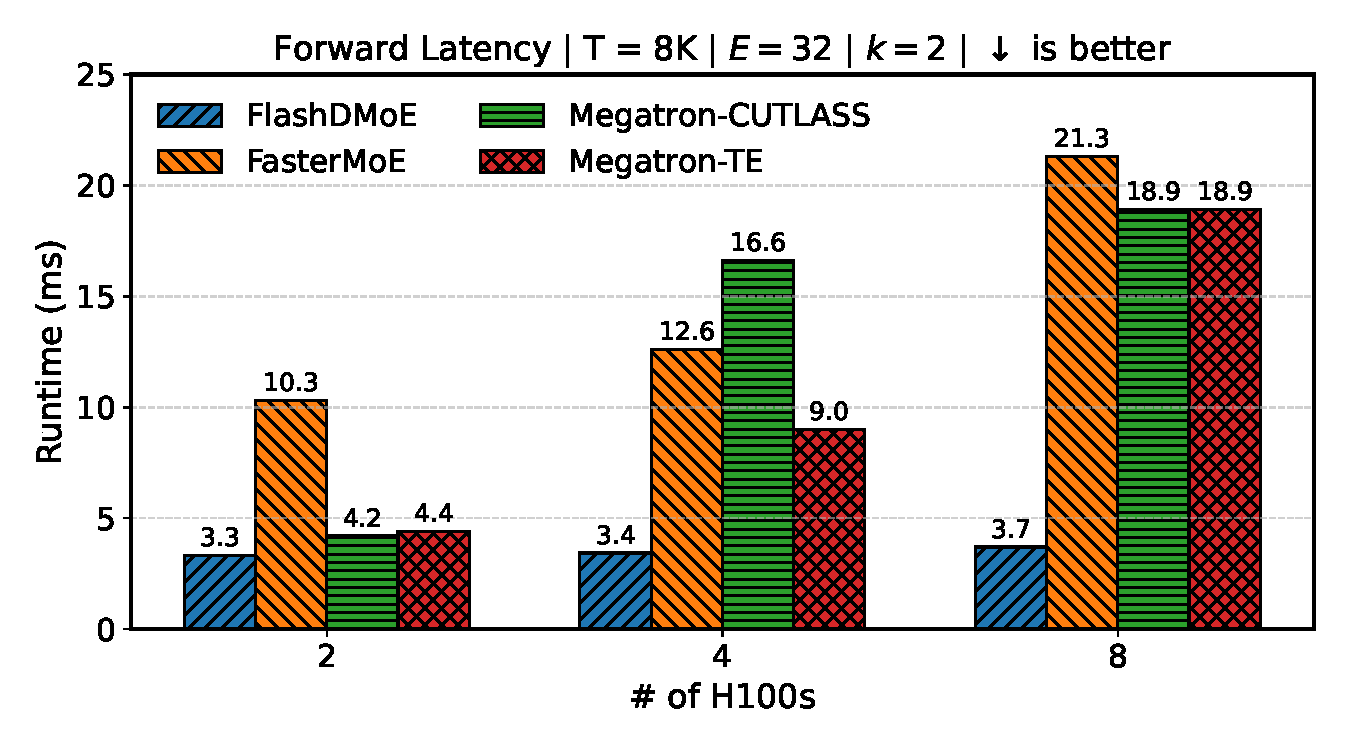
\includegraphics[width=\linewidth, keepaspectratio]{figures/scaling_gpus_8}
        \caption{Weak Scaling across GPUs}
        \label{sub:weak_scaling}
    \end{subfigure}
    \begin{subfigure}{0.4\textwidth}
        \centering
        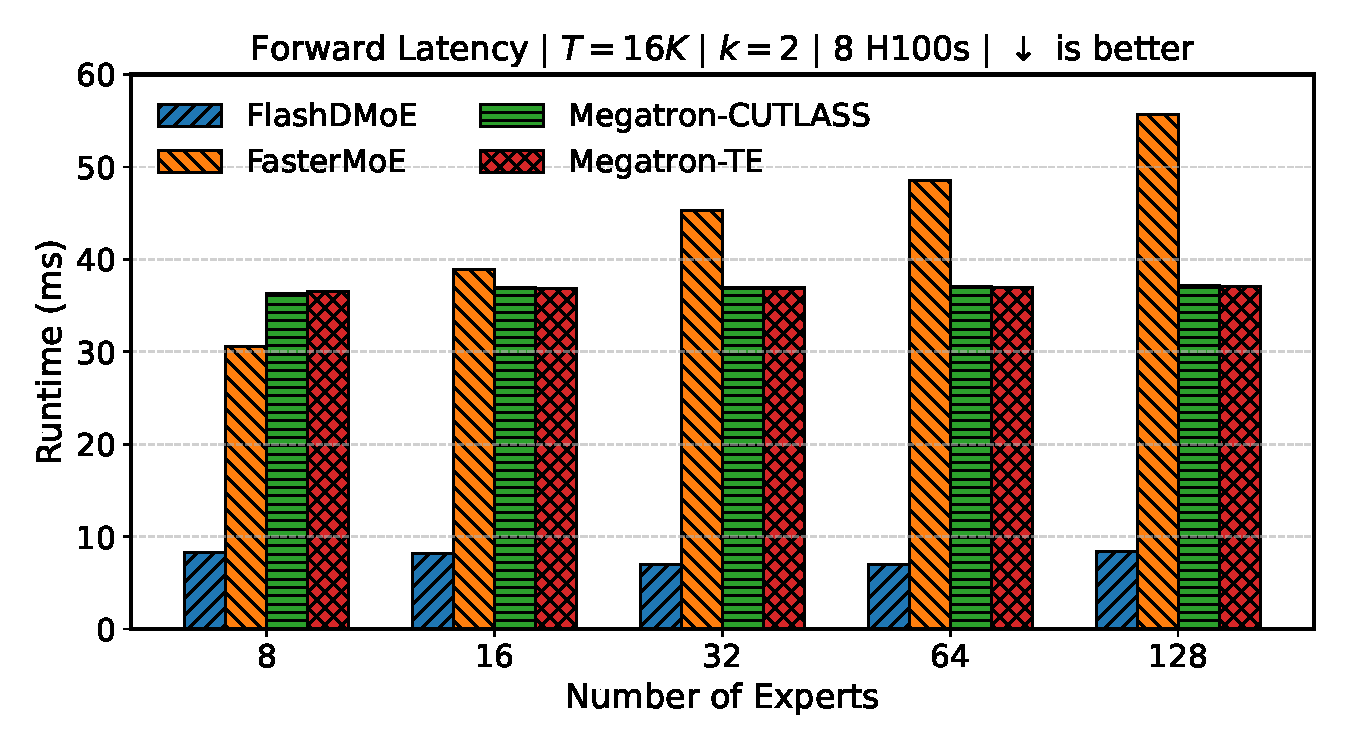
\includegraphics[width=\linewidth, keepaspectratio]{figures/scaling_experts_8}
        \caption{Expert Scalability}
        \label{sub:experts}
    \end{subfigure}
    \caption{\emph{FlashDMoE} demonstrating
        (a) improved SM Utilization
        (b) lower latency for longer token sequences
        (c) approximately ideal weak scaling and
        (c) ideal expert scalability.
    }
    \label{fig:perf_contributions}
\end{figure}
To overcome these fundamental inefficiencies in state-of-the-art MoE models, we develop \sysname, where we
integrate all DMoE computation and communication tasks into a single persistent GPU kernel,
namely a kernel that remains active for the entirety of the MoE operator (Figure~\ref{fig:intro} bottom left).
Instead of multiple kernel launches coordinated by the CPU, \sysname requires launching only one kernel,
significantly reducing the involvement of the CPU\@.
Within the fused kernel, \sysname implements a reactive programming model to achieve
fine-grained parallelism and loosely coupled, non-blocking execution among tens of thousands of GPU threads.
This design enables \sysname to efficiently utilize GPU resources by reducing idle time.
\subsection{Warp Specialization and Tile Parallelism.}\label{subsec:wstp}
\begin{figure}[!ht]
    \centering
    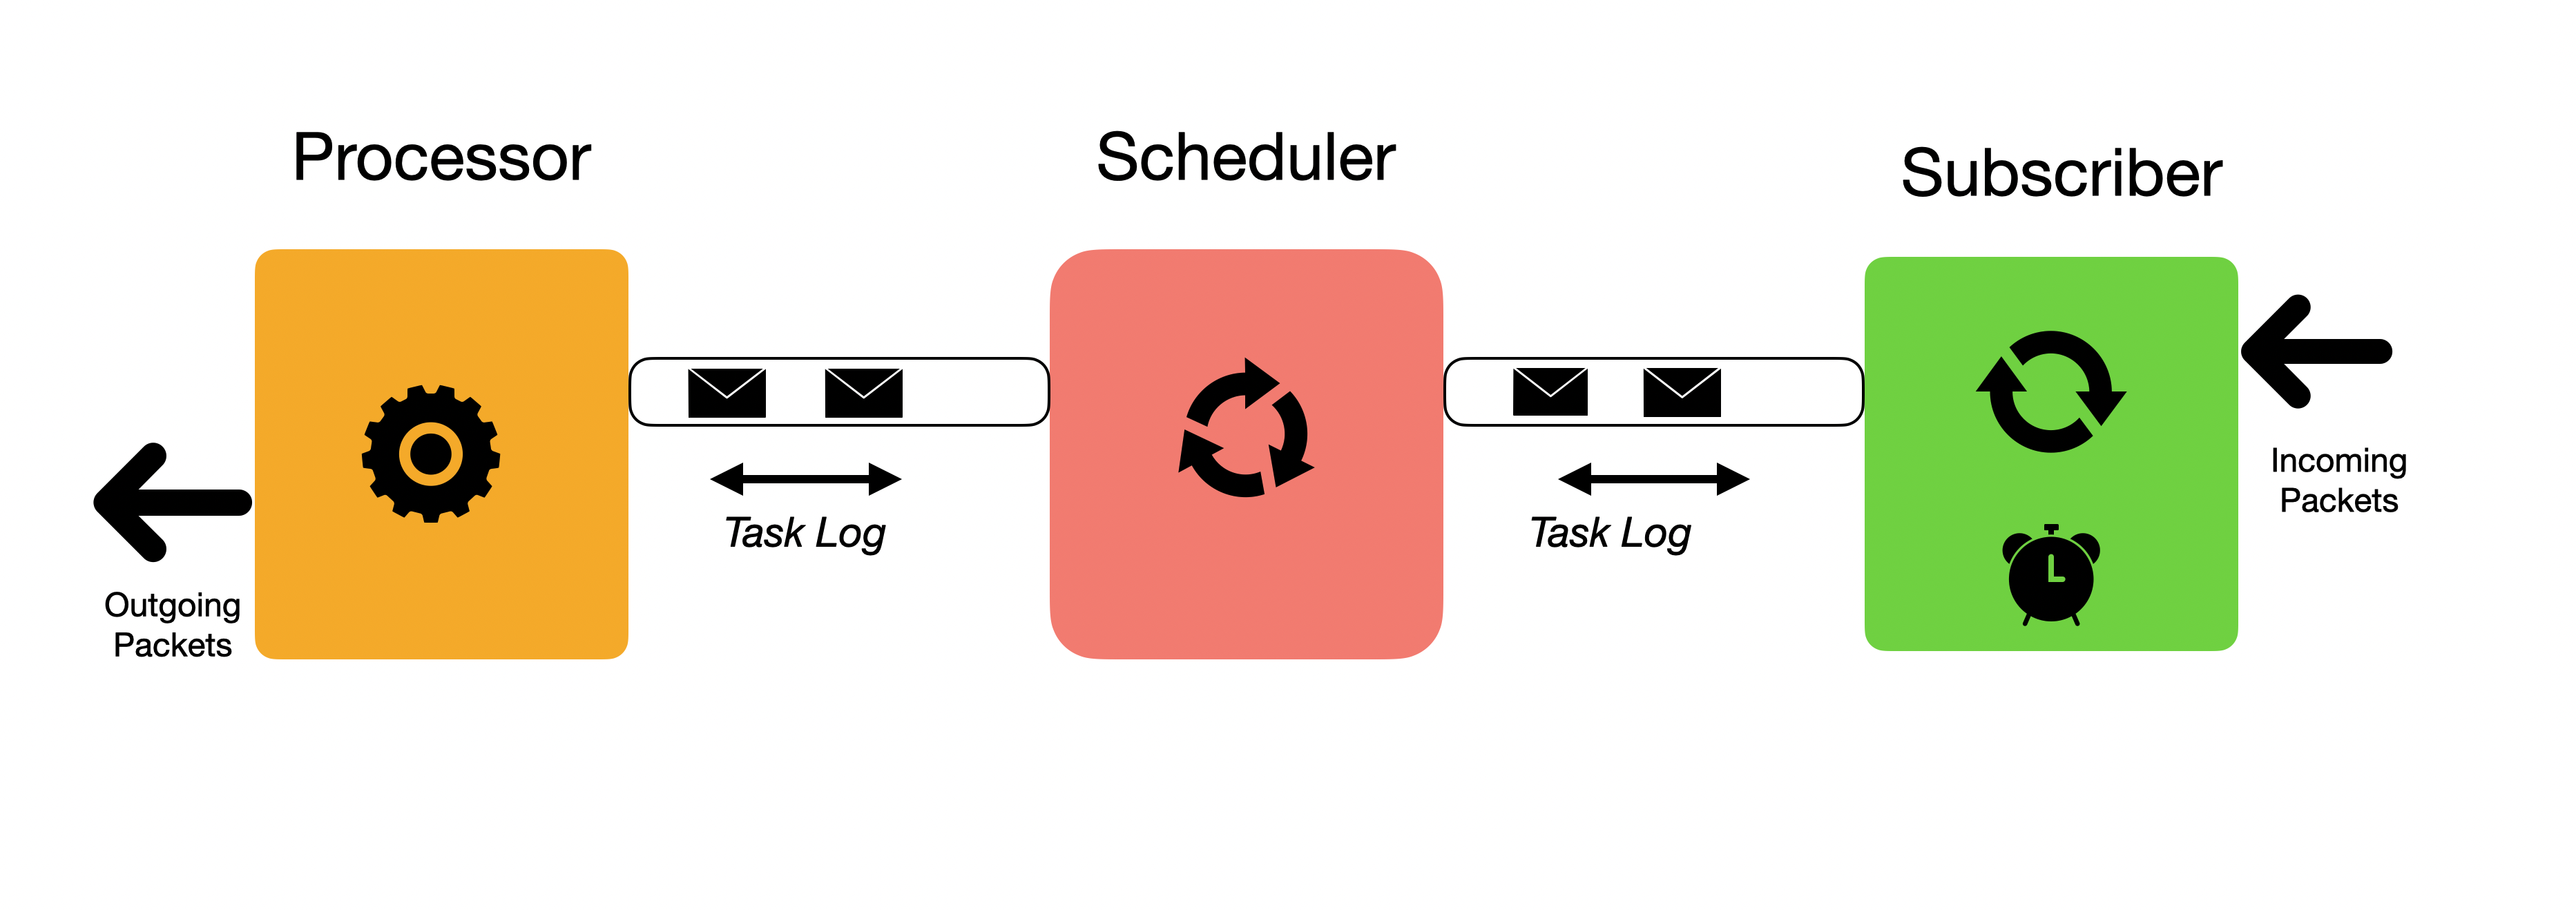
\includegraphics[width=0.98\textwidth, keepaspectratio]{figures/flash_actors}
    \caption{\sysname Actors. The \textcolor{LimeGreen}{Subscriber} observes received remote \emph{packets}
    (blob of tiles), decodes them into \emph{tasks} and notifies the scheduler of the enqueued tasks.
    We assign three CUDA warps to this role.
    The \textcolor{Salmon}{Scheduler} maintains a \emph{ready queue} of \textcolor{Orange}{Processors}
    from which it schedules tasks. The \textcolor{Yellow}{Processors} performs the operation encoded in its task
    descriptor and eagerly communicates its output, if necessary.}
    \label{fig:flash_actors}
\end{figure}
\sysname implements \emph{tile-level parallelism},
meaning it partitions input token matrices into statically sized, \emph{independent}
tensors, called \emph{tiles},
which are processed concurrently by a set of GPU thread warps comprising a
\textbf{C}ooperative \textbf{T}hread \textbf{A}rray (CTA) or thread block.
We specialize every thread block, except one, as \emph{processors} to perform computation and
remote data transfers.
In addition, we designate a dedicated Operating System (OS) block (4 warps) to perform administrative tasks of
(1) scheduling computational work to processors (\emph{scheduler}),
and (2) decoding computational tasks from messages received from other GPUs (\emph{subscriber}).
This design allows \sysname to dynamically assign tasks to GPU blocks based on \emph{readiness},
ensuring that no GPU SM remains idle throughout the lifetime of the DMoE operator.
\sysname selects tile dimensions to maximize GPU arithmetic intensity
while still benefitting from a high-degree of parallelism.
\subsection{Asynchronous and payload-efficient communication.}\label{subsec:asynchronous-and-payload-efficient-communication.}
\begin{figure}[!ht]
    \centering
    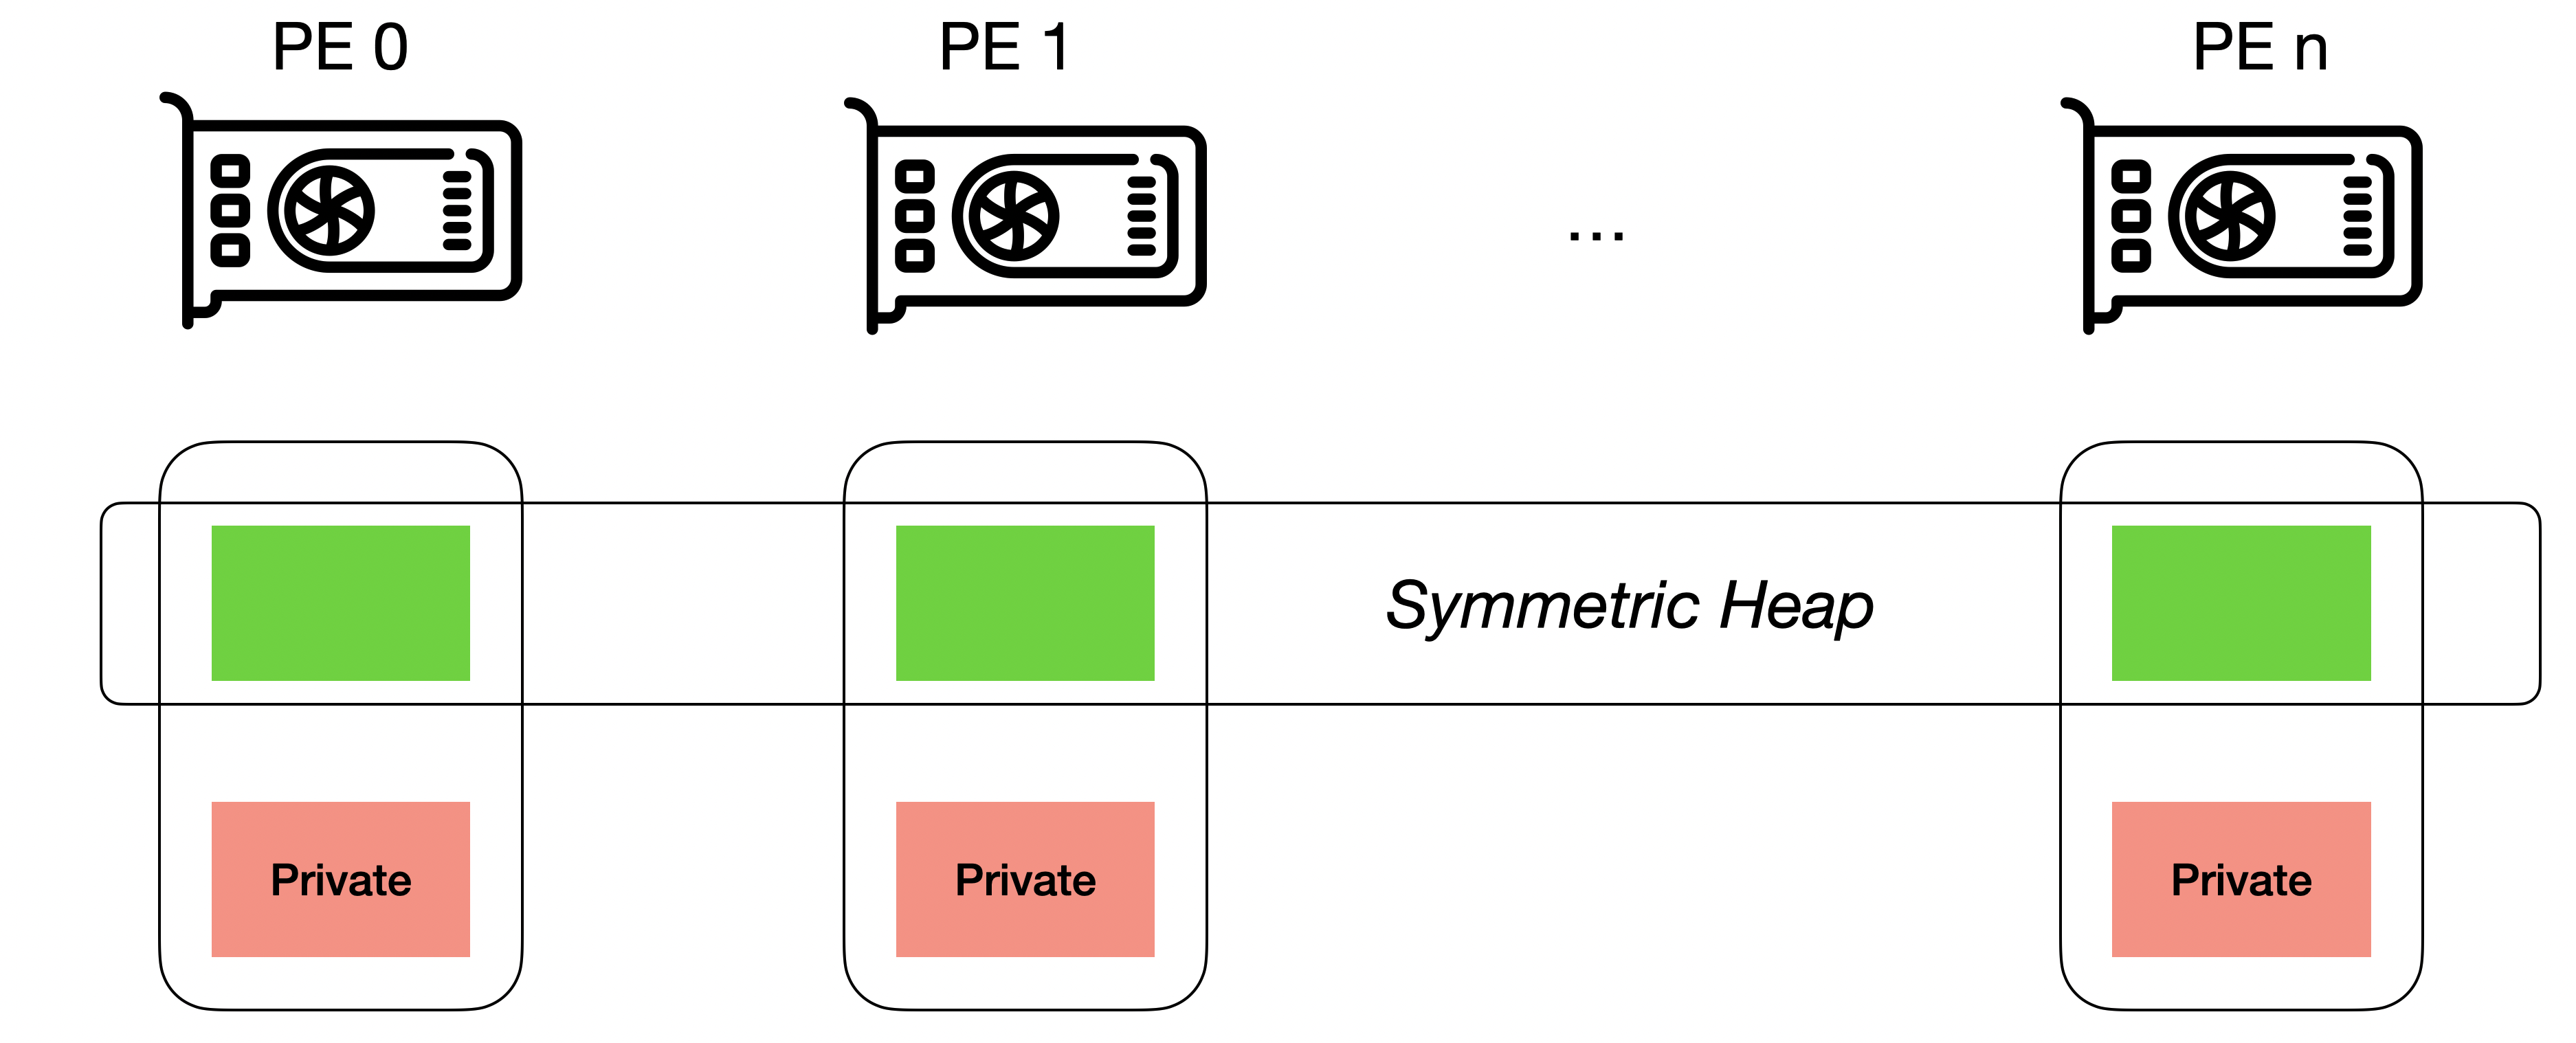
\includegraphics[width=0.98\textwidth, keepaspectratio]{figures/pgas}
    \caption{Depiction of a Partitioned Global Adress Space (PGAS)~\cite{10.1145/1278177.1278183}
        across a \textit{team} of \textbf{P}rocessing \textbf{E}lements (PEs). The symmetric heap is an
    unifromly sized memroy region resident on each PE and accessible by every other PE via one-sided
    \textbf{D}irect \textbf{M}emory \textbf{A}ccess (DMA) or \textbf{R}emote DMA (RDMA) operations.}
    \label{fig:pgas}
\end{figure}
By redesigning the MoE operator from the ground up,
\sysname resolves fundamental inefficiencies inherent in the conventional MoE execution pipeline.
One notable inefficiency is token padding during communication.
To simplify programming complexity and due to symmetry constraints of collective communication APIs,
existing implementations have to zero-pad token payloads to match predefined buffer sizes.
This occurs when tokens are asymmetrically routed to experts, resulting in GPUs receiving much less than the expected
capacity.
However, these null payloads waste communication bandwidth, bloat data transfer latency and may lead to
unnecessary computations on null matrices in some implementations.
\sysname introduces \emph{payload-efficient} communication by sending non-padded tokens only to
GPUs with actively selected experts, conserving both communication and computational resources.
\subsection{Technical Challenges}\label{subsec:technical-challenges}
Realizing the single-kernel design of \sysname required
solving several technical challenges to achieve high performance:
(1) lightweight computational dependency management; (2)
navigating optimal SM occupancy configurations; (3) implementing in-device BLAS operations;
(4) minimizing inter- and intra-device synchronization overheads; (5) implementing transfer-awareness by leveraging
DMA over Unified Virtual Addressing (UVA) when available.
In addressing these challenges, \sysname's design presents a
radical departure from traditional synchronous \alltoall collectives,
where GPUs exhibit significant idle time during layer execution.
For device-initiated communication,
\sysname uses NVSHMEM~\cite{nvshm} to establish a global address space across all GPUs to
achieve the aforementioned Direct Memory Access (DMA) or Remote DMA (RDMA) communication.
For in-device BLAS, \sysname develops custom high-performance GEMM operations via CUTLASS~\cite{Thakkar_CUTLASS_2023}.
\subsection{Research Papers}\label{subsec:research-papers}
This thesis comprises a first-author publication at ACM SIGMETRICS'24~\cite{10.1145/3725536.3725539}
and another first-author submission in review at NeurIPS \('25\)~\cite{flasharxiv}.
\subsection{Code Artifact}\label{subsec:code-artifact}
We open source the code and steps to reproduce all results contained in this thesis at
\url{https://github.com/osayamenja/Kleos/tree/main/csrc/include/kleos/moe}

